\documentclass[12pt]{report}
\usepackage[utf8]{inputenc}
\usepackage[russian]{babel}
%\usepackage[14pt]{extsizes}
\usepackage{listings}
\usepackage{graphicx}
\usepackage{amsmath,amsfonts,amssymb,amsthm,mathtools} 
\usepackage{pgfplots}
\usepackage{filecontents}
\usepackage{float}
\usepackage{comment}
\usepackage{indentfirst}
\usepackage{eucal}
\usepackage{enumitem}
%s\documentclass[openany]{book}
\frenchspacing

\usepackage{indentfirst} % Красная строка

\usetikzlibrary{datavisualization}
\usetikzlibrary{datavisualization.formats.functions}

\usepackage{amsmath}


% Для листинга кода:
\lstset{ %
	language=c,                 % выбор языка для подсветки (здесь это С)
	basicstyle=\small\sffamily, % размер и начертание шрифта для подсветки кода
	numbers=left,               % где поставить нумерацию строк (слева\справа)
	numberstyle=\tiny,           % размер шрифта для номеров строк
	stepnumber=1,                   % размер шага между двумя номерами строк
	numbersep=5pt,                % как далеко отстоят номера строк от подсвечиваемого кода
	showspaces=false,            % показывать или нет пробелы специальными отступами
	showstringspaces=false,      % показывать или нет пробелы в строках
	showtabs=false,             % показывать или нет табуляцию в строках
	frame=single,              % рисовать рамку вокруг кода
	tabsize=2,                 % размер табуляции по умолчанию равен 2 пробелам
	captionpos=t,              % позиция заголовка вверху [t] или внизу [b] 
	breaklines=true,           % автоматически переносить строки (да\нет)
	breakatwhitespace=false, % переносить строки только если есть пробел
	escapeinside={\#*}{*)}   % если нужно добавить комментарии в коде
}


\usepackage[left=2cm,right=2cm, top=2cm,bottom=2cm,bindingoffset=0cm]{geometry}
% Для измененных титулов глав:
\usepackage{titlesec, blindtext, color} % подключаем нужные пакеты
\definecolor{gray75}{gray}{0.75} % определяем цвет
\newcommand{\hsp}{\hspace{20pt}} % длина линии в 20pt
% titleformat определяет стиль
\titleformat{\section}[hang]{\Huge\bfseries}{\thechapter\hsp\textcolor{gray75}{|}\hsp}{0pt}{\Huge\bfseries}


% plot
\usepackage{pgfplots}
\usepackage{filecontents}
\usetikzlibrary{datavisualization}
\usetikzlibrary{datavisualization.formats.functions}

\begin{document}
	%\def\sectionname{} % убирает "Глава"
	\thispagestyle{empty}
	\begin{titlepage}
		\noindent \begin{minipage}{0.15\textwidth}
			
\includegraphics[width=\linewidth]{b_logo}
		\end{minipage}
		\noindent\begin{minipage}{0.9\textwidth}\centering
			\textbf{Министерство науки и высшего образования Российской Федерации}\\
			\textbf{Федеральное государственное бюджетное образовательное учреждение высшего образования}\\
			\textbf{~~~«Московский государственный технический университет имени Н.Э.~Баумана}\\
			\textbf{(национальный исследовательский университет)»}\\
			\textbf{(МГТУ им. Н.Э.~Баумана)}
		\end{minipage}
		
		\noindent\rule{18cm}{3pt}
		\newline\newline
		\noindent ФАКУЛЬТЕТ $\underline{\text{«Информатика и системы управления»}}$ \newline\newline
		\noindent КАФЕДРА $\underline{\text{«Программное обеспечение ЭВМ и информационные технологии»}}$\newline\newline\newline\newline\newline
		
		\begin{center}
			\noindent\begin{minipage}{1.1\textwidth}\centering
				\Large\textbf{Отчет по лабораторной работе №14}\newline
				\textbf{по дисциплине <<Функциональное и логическое}\newline
				\textbf{~~~программирование>>}\newline\newline
			\end{minipage}
		\end{center}
		
		\noindent\textbf{Тема} $\underline{\text{Использование правил в программе на Prolog}}$\newline\newline
		\noindent\textbf{Студент} $\underline{\text{Варламова Е. А.~~~~~~~~~~~~~~~~~~~~~~~~~~~~~~~~~~~~~~~~~~~~~~~~~~~~~~~~~~~~~~~~~}}$\newline\newline
		\noindent\textbf{Группа} $\underline{\text{ИУ7-61Б~~~~~~~~~~~~~~~~~~~~~~~~~~~~~~~~~~~~~~~~~~~~~~~~~~~~~~~~~~~~~~~~~~~~~~~~~}}$\newline\newline
		\noindent\textbf{Оценка (баллы)} $\underline{\text{~~~~~~~~~~~~~~~~~~~~~~~~~~~~~~~~~~~~~~~~~~~~~~~~~~~~~~~~~~~~~~~~~~~~~~~~}}$\newline\newline
		\noindent\textbf{Преподаватель} $\underline{\text{Толпинская Н.Б., Строганов Ю. В.~~~~~~~~~~~~~~~~~~~~~~~~~~}}$\newline\newline\newline
		
		\begin{center}
			\vfill
			Москва~---~\the\year
			~г.
		\end{center}
	\end{titlepage}
\section*{Задание}
Создать базу знаний: «ПРЕДКИ», позволяющую наиболее эффективным способом (за меньшее количество шагов, что обеспечивается меньшим количеством предложений БЗ - правил), и используя разные варианты (примеры) одного вопроса, определить (указать: какой вопрос для какого варианта):
\begin{enumerate}
    \item по имени субъекта определить всех его бабушек (предки 2-го колена),
    \item по имени субъекта определить всех его дедушек (предки 2-го колена),
    \item по имени субъекта определить всех его бабушек и дедушек (предки 2-го
колена),
    \item по имени субъекта определить его бабушку по материнской линии (предки 2-го колена),
    \item по имени субъекта определить его бабушку и дедушку по материнской линии (предки 2-го колена).
\end{enumerate}
Минимизировать количество правил и количество вариантов вопросов. Использовать конъюнктивные правила и простой вопрос.

\chapter*{Решение}
\begin{lstlisting}
domains
name = symbol.
gender = symbol.

predicates
hasGender(name, symbol).
pred(name, name).
grandpred(name, gender, name, gender).

clauses
grandpred(Name, PG, GPName, GPG) :- pred(X, Name), hasGender(X, PG), pred(GPName, X), hasGender(GPName, GPG).
pred(buri, odin).
pred(bolthorn, bestla).
pred(borr, odin).
pred(bestla, odin).
pred(fjorginn, frigg).
pred(fjorgyn, frigg).
pred(odin, thor).
pred(jord, thor).
pred(odin, heimdall).
pred(nine, heimdall).
pred(odin, tyr).
pred(odin, baldr).
pred(frigg, baldr).
pred(odin, hed).
pred(frigg, hed).
pred(farabuti, loki).
pred(laufeya, loki).
pred(loki, fenrir).
pred(loki, hel).
pred(loki, jormungandr).

hasgender(loki, m).
hasgender(odin, m).
hasgender(frigg, f).
hasgender(jord, f).
hasgender(fjorginn, m).
hasgender(fjorgyn, f).
hasgender(nine, f).
hasgender(borr, m).
hasgender(bestla, f).
hasgender(bolthorn, m).
hasgender(buri, m).
hasgender(farabuti, m).
hasgender(laufeya, f).
hasgender(tyr, m).
hasgender(baldr, m).
hasgender(hed, m).
hasgender(hel, f).
hasgender(fenrir, m).
hasgender(jormungandr, m).

goal
%grandpred(baldr, _, X, f).
%grandpred(baldr, _, X, m).
%grandpred(baldr, _, X, _).
%grandpred(baldr, f, X, f).
%grandpred(baldr, f, X, _).
\end{lstlisting}


Порядок формирования результата для 1-го вопроса:

\begin{figure}[H]
	\centering
	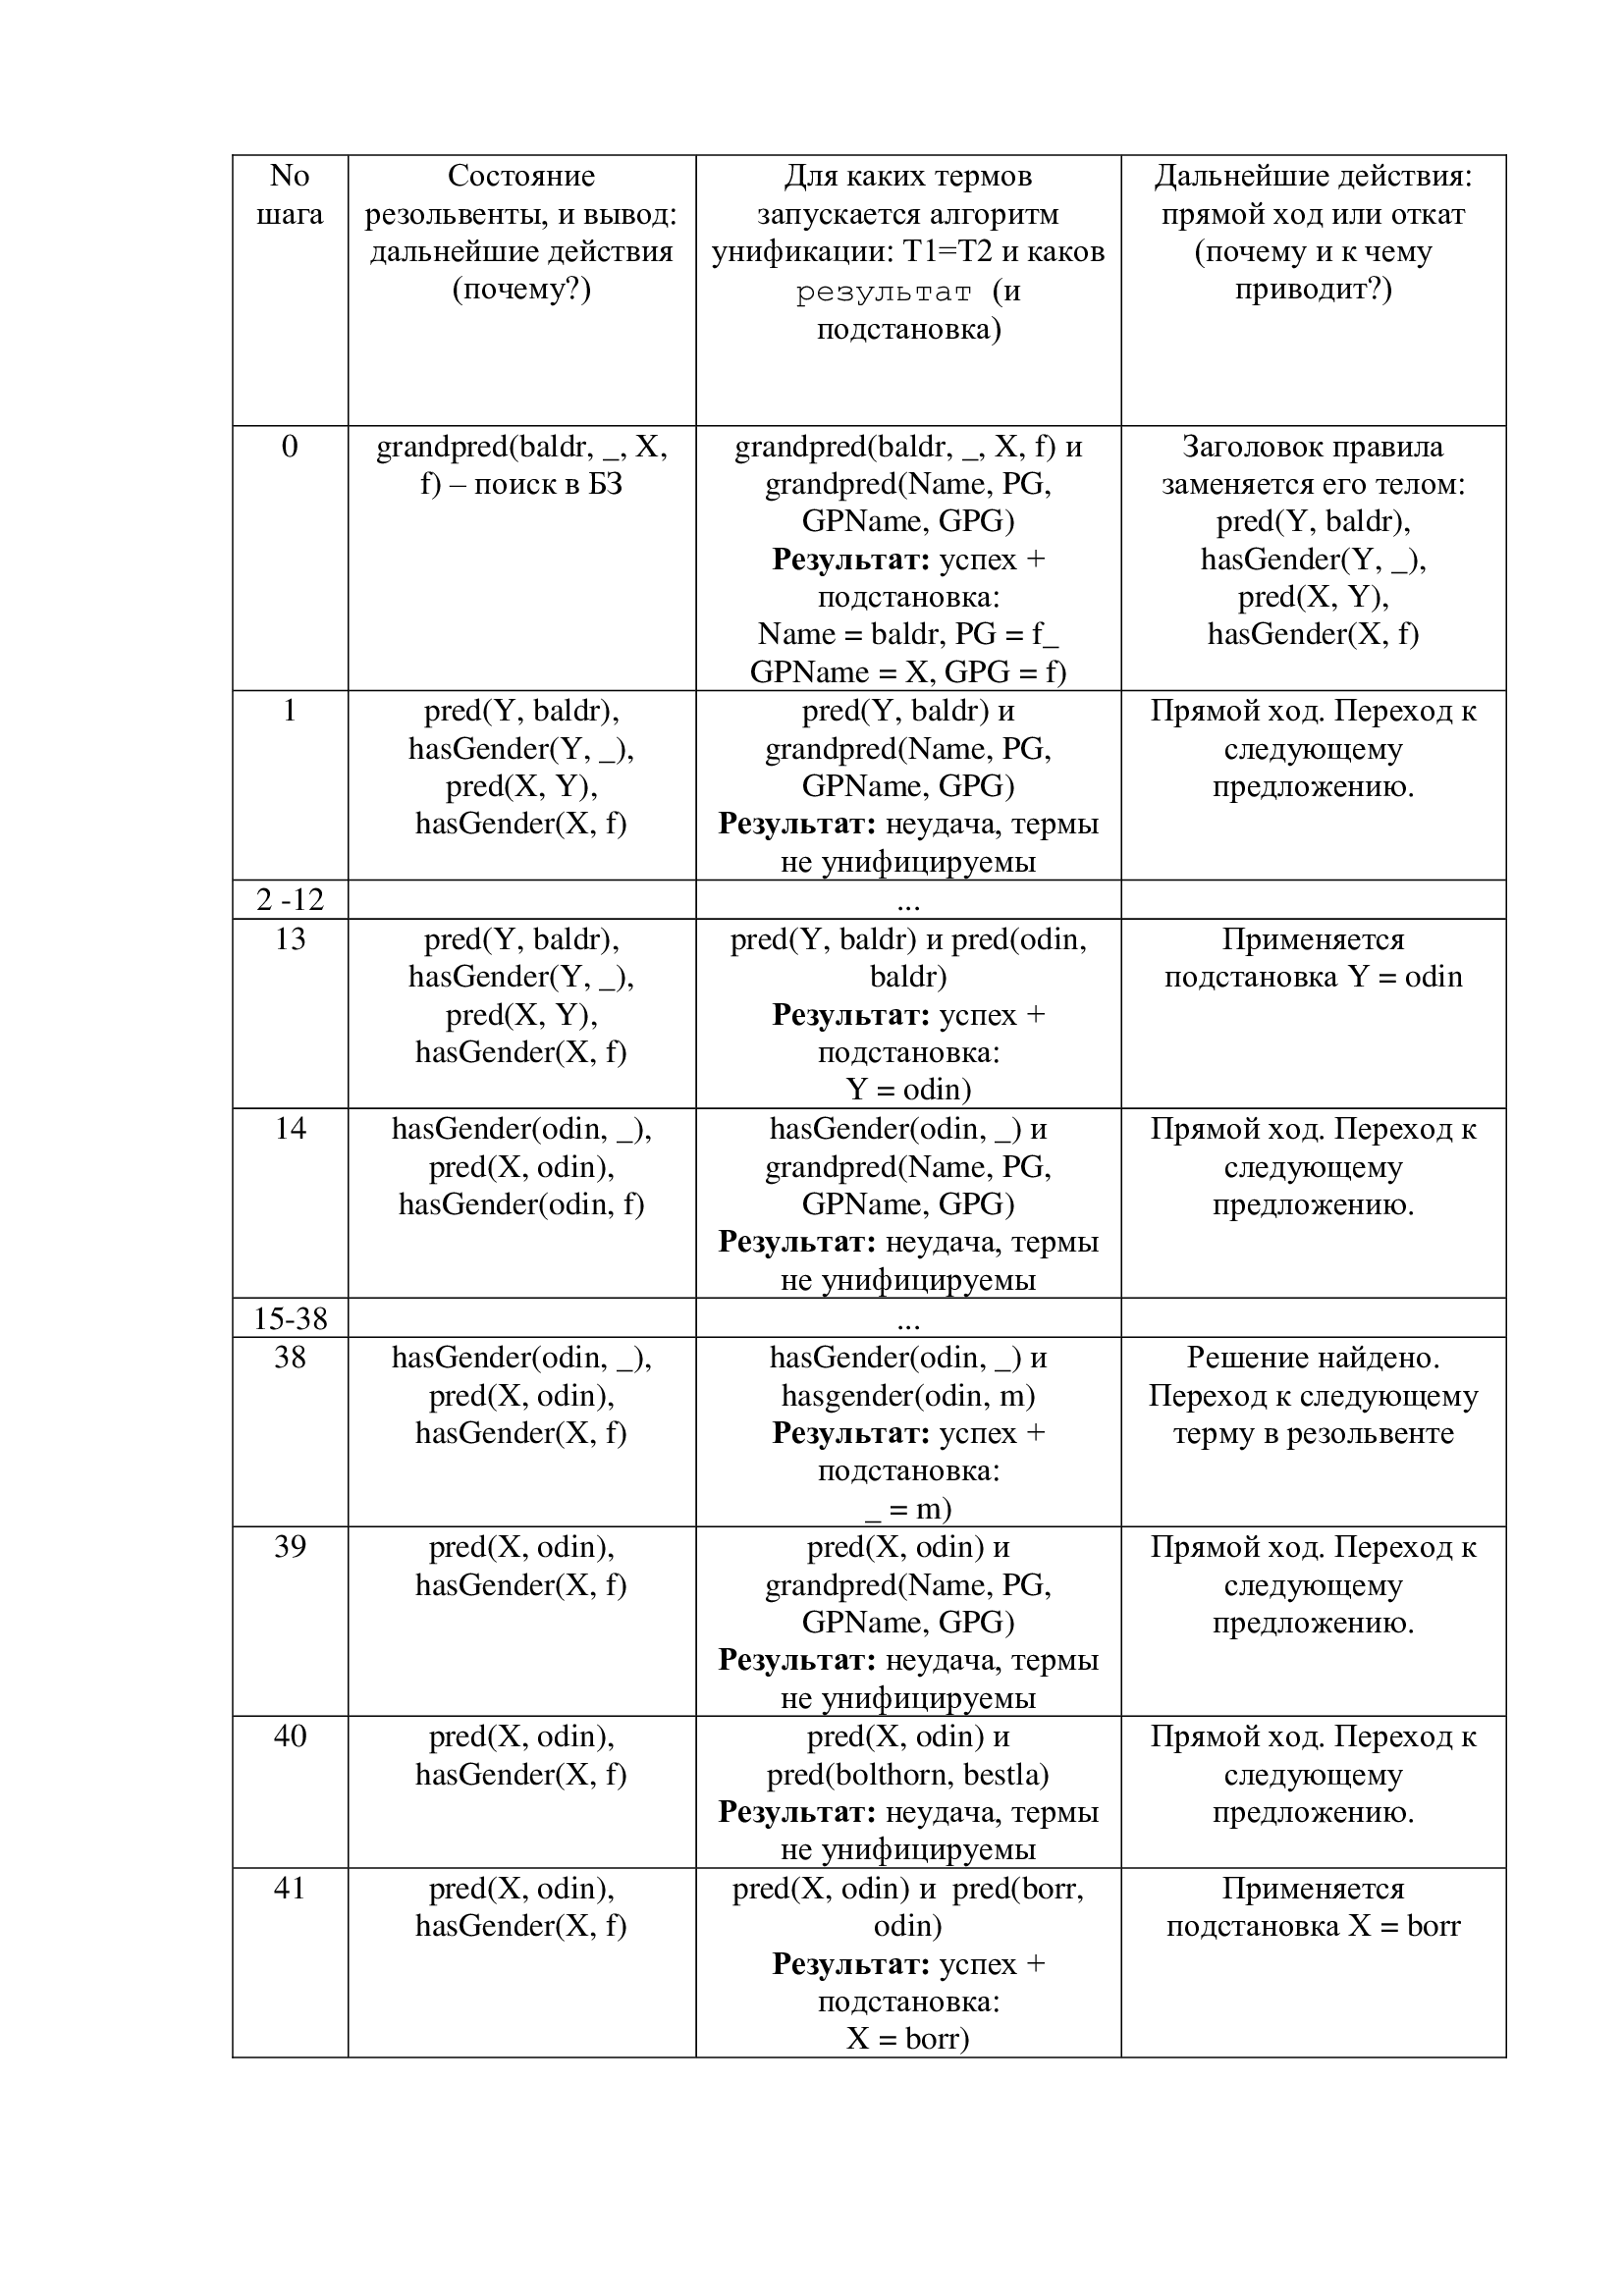
\includegraphics[scale=0.32]{0.png}
	\label{fig:1}
\end{figure}

\begin{figure}[H]
	\centering
	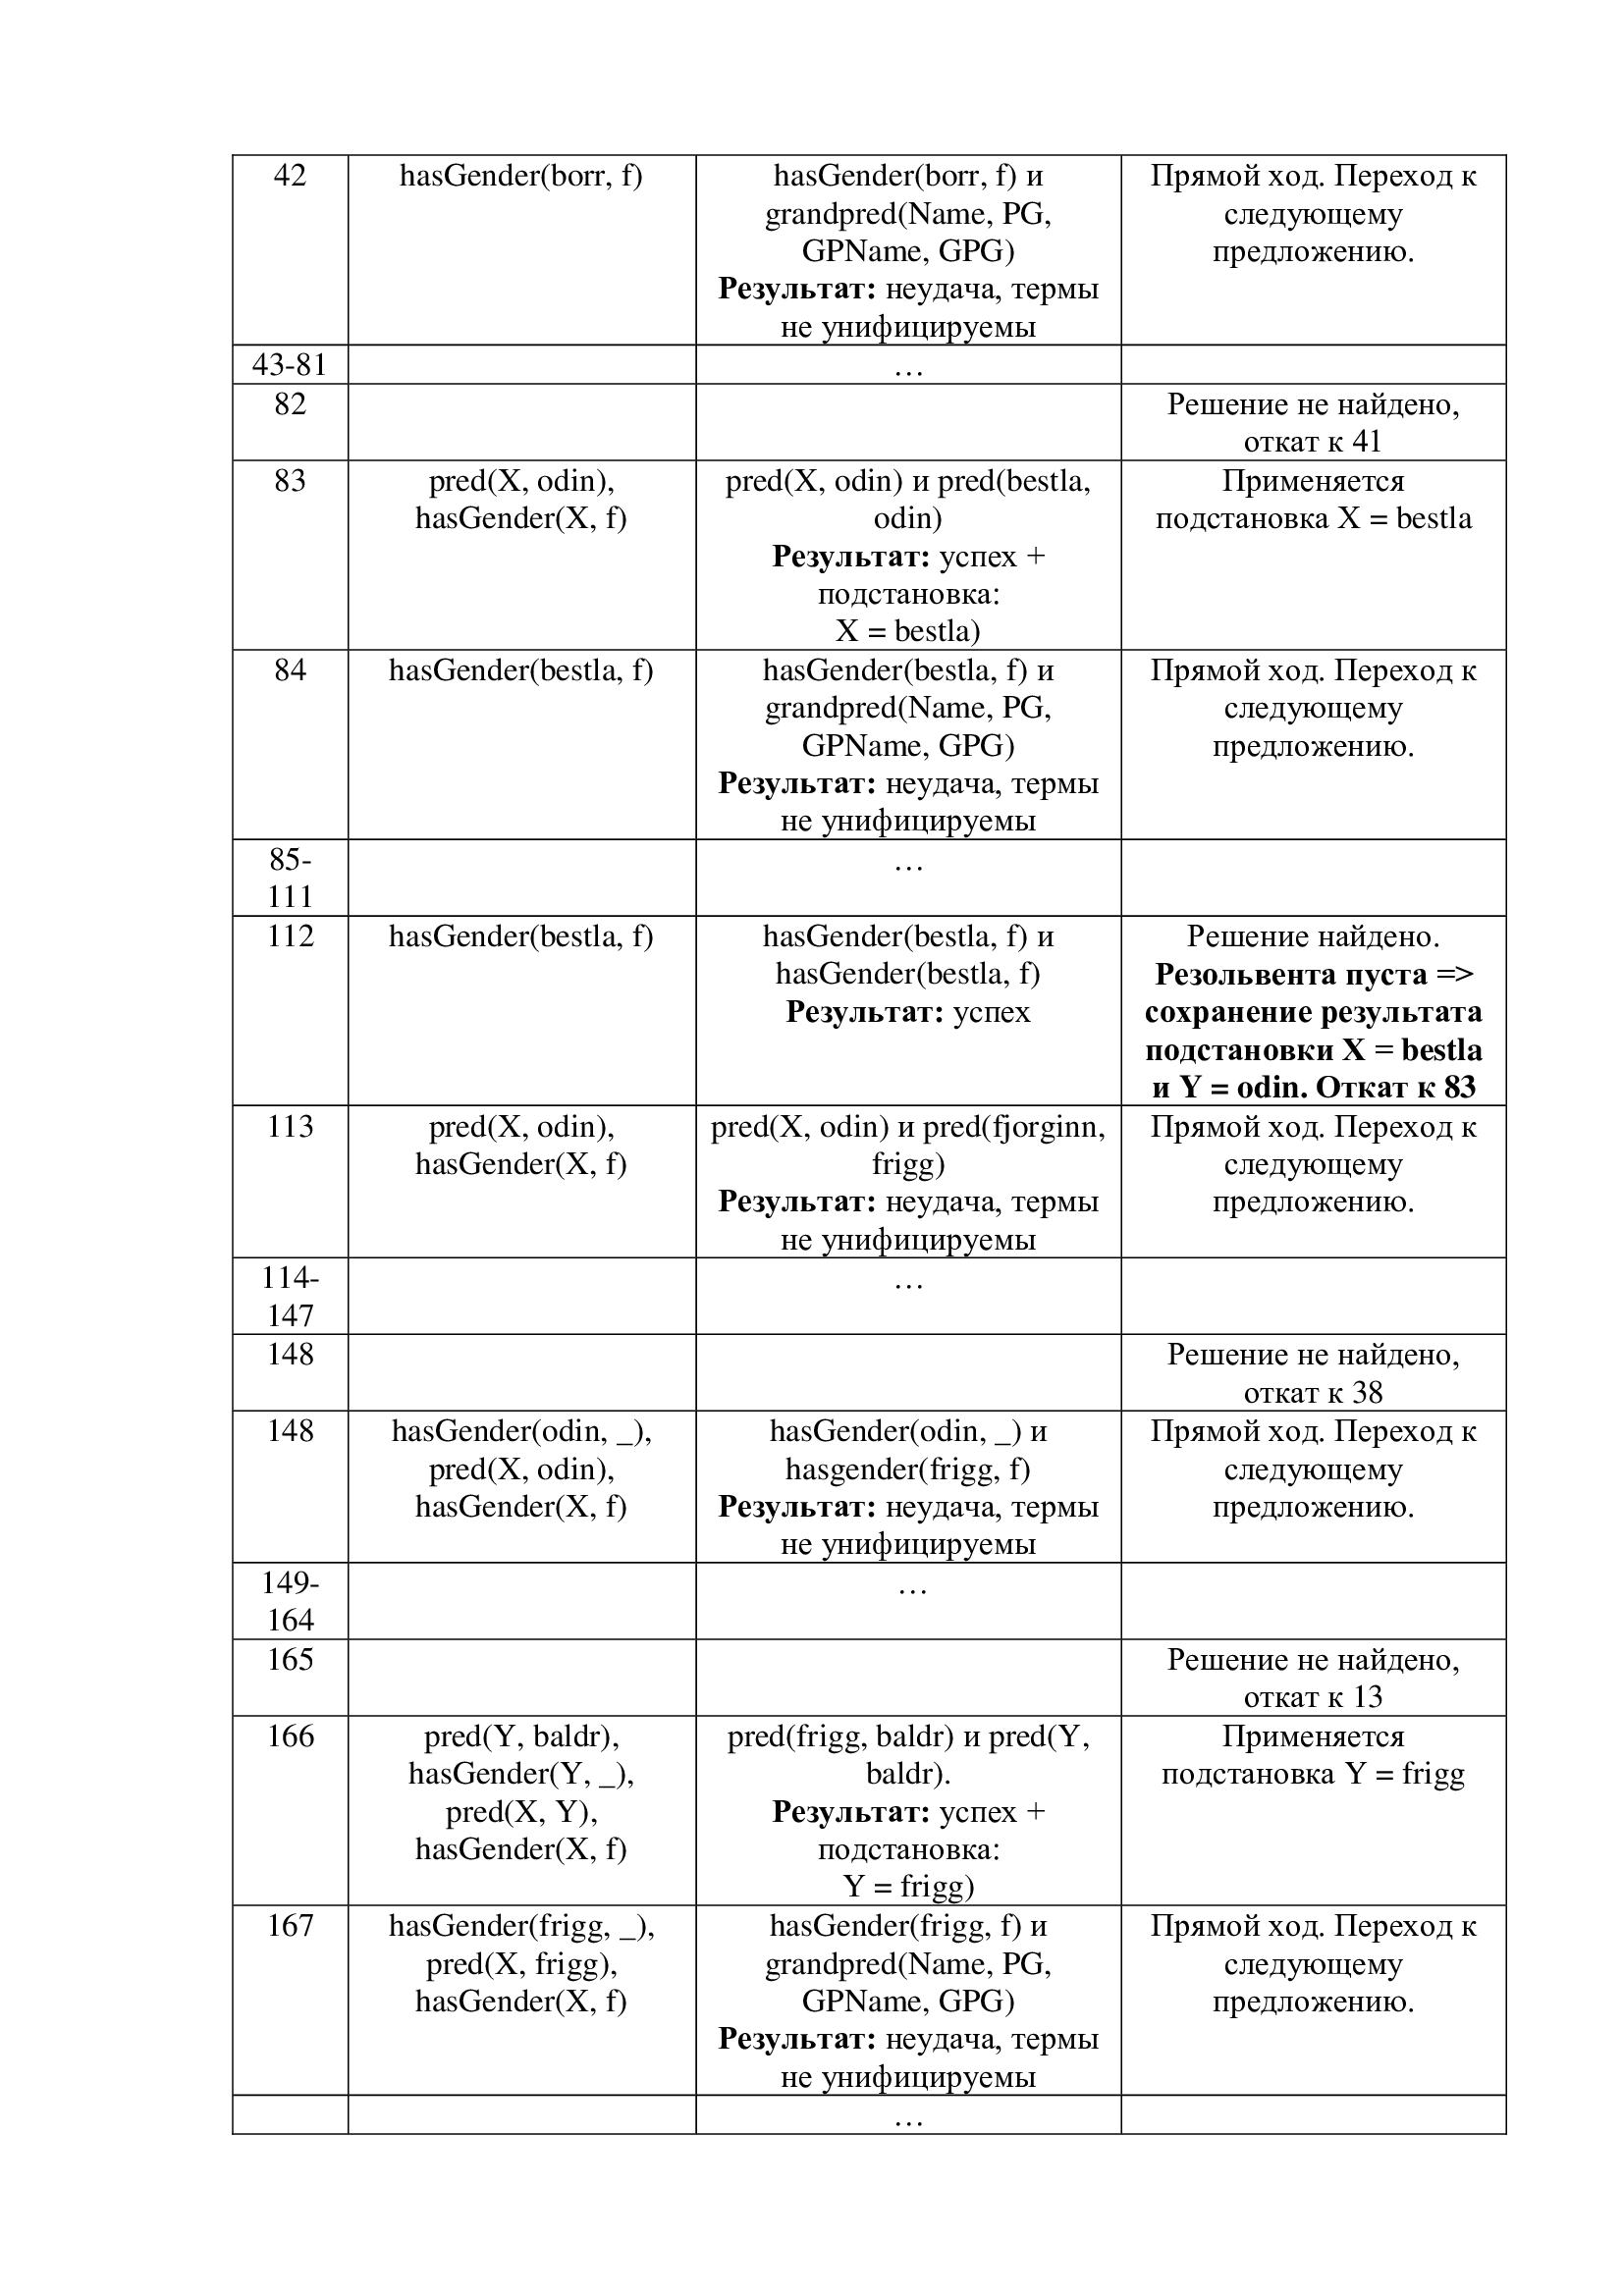
\includegraphics[scale=0.32]{1.png}
	\label{fig:1}
\end{figure}

\begin{figure}[H]
	\centering
	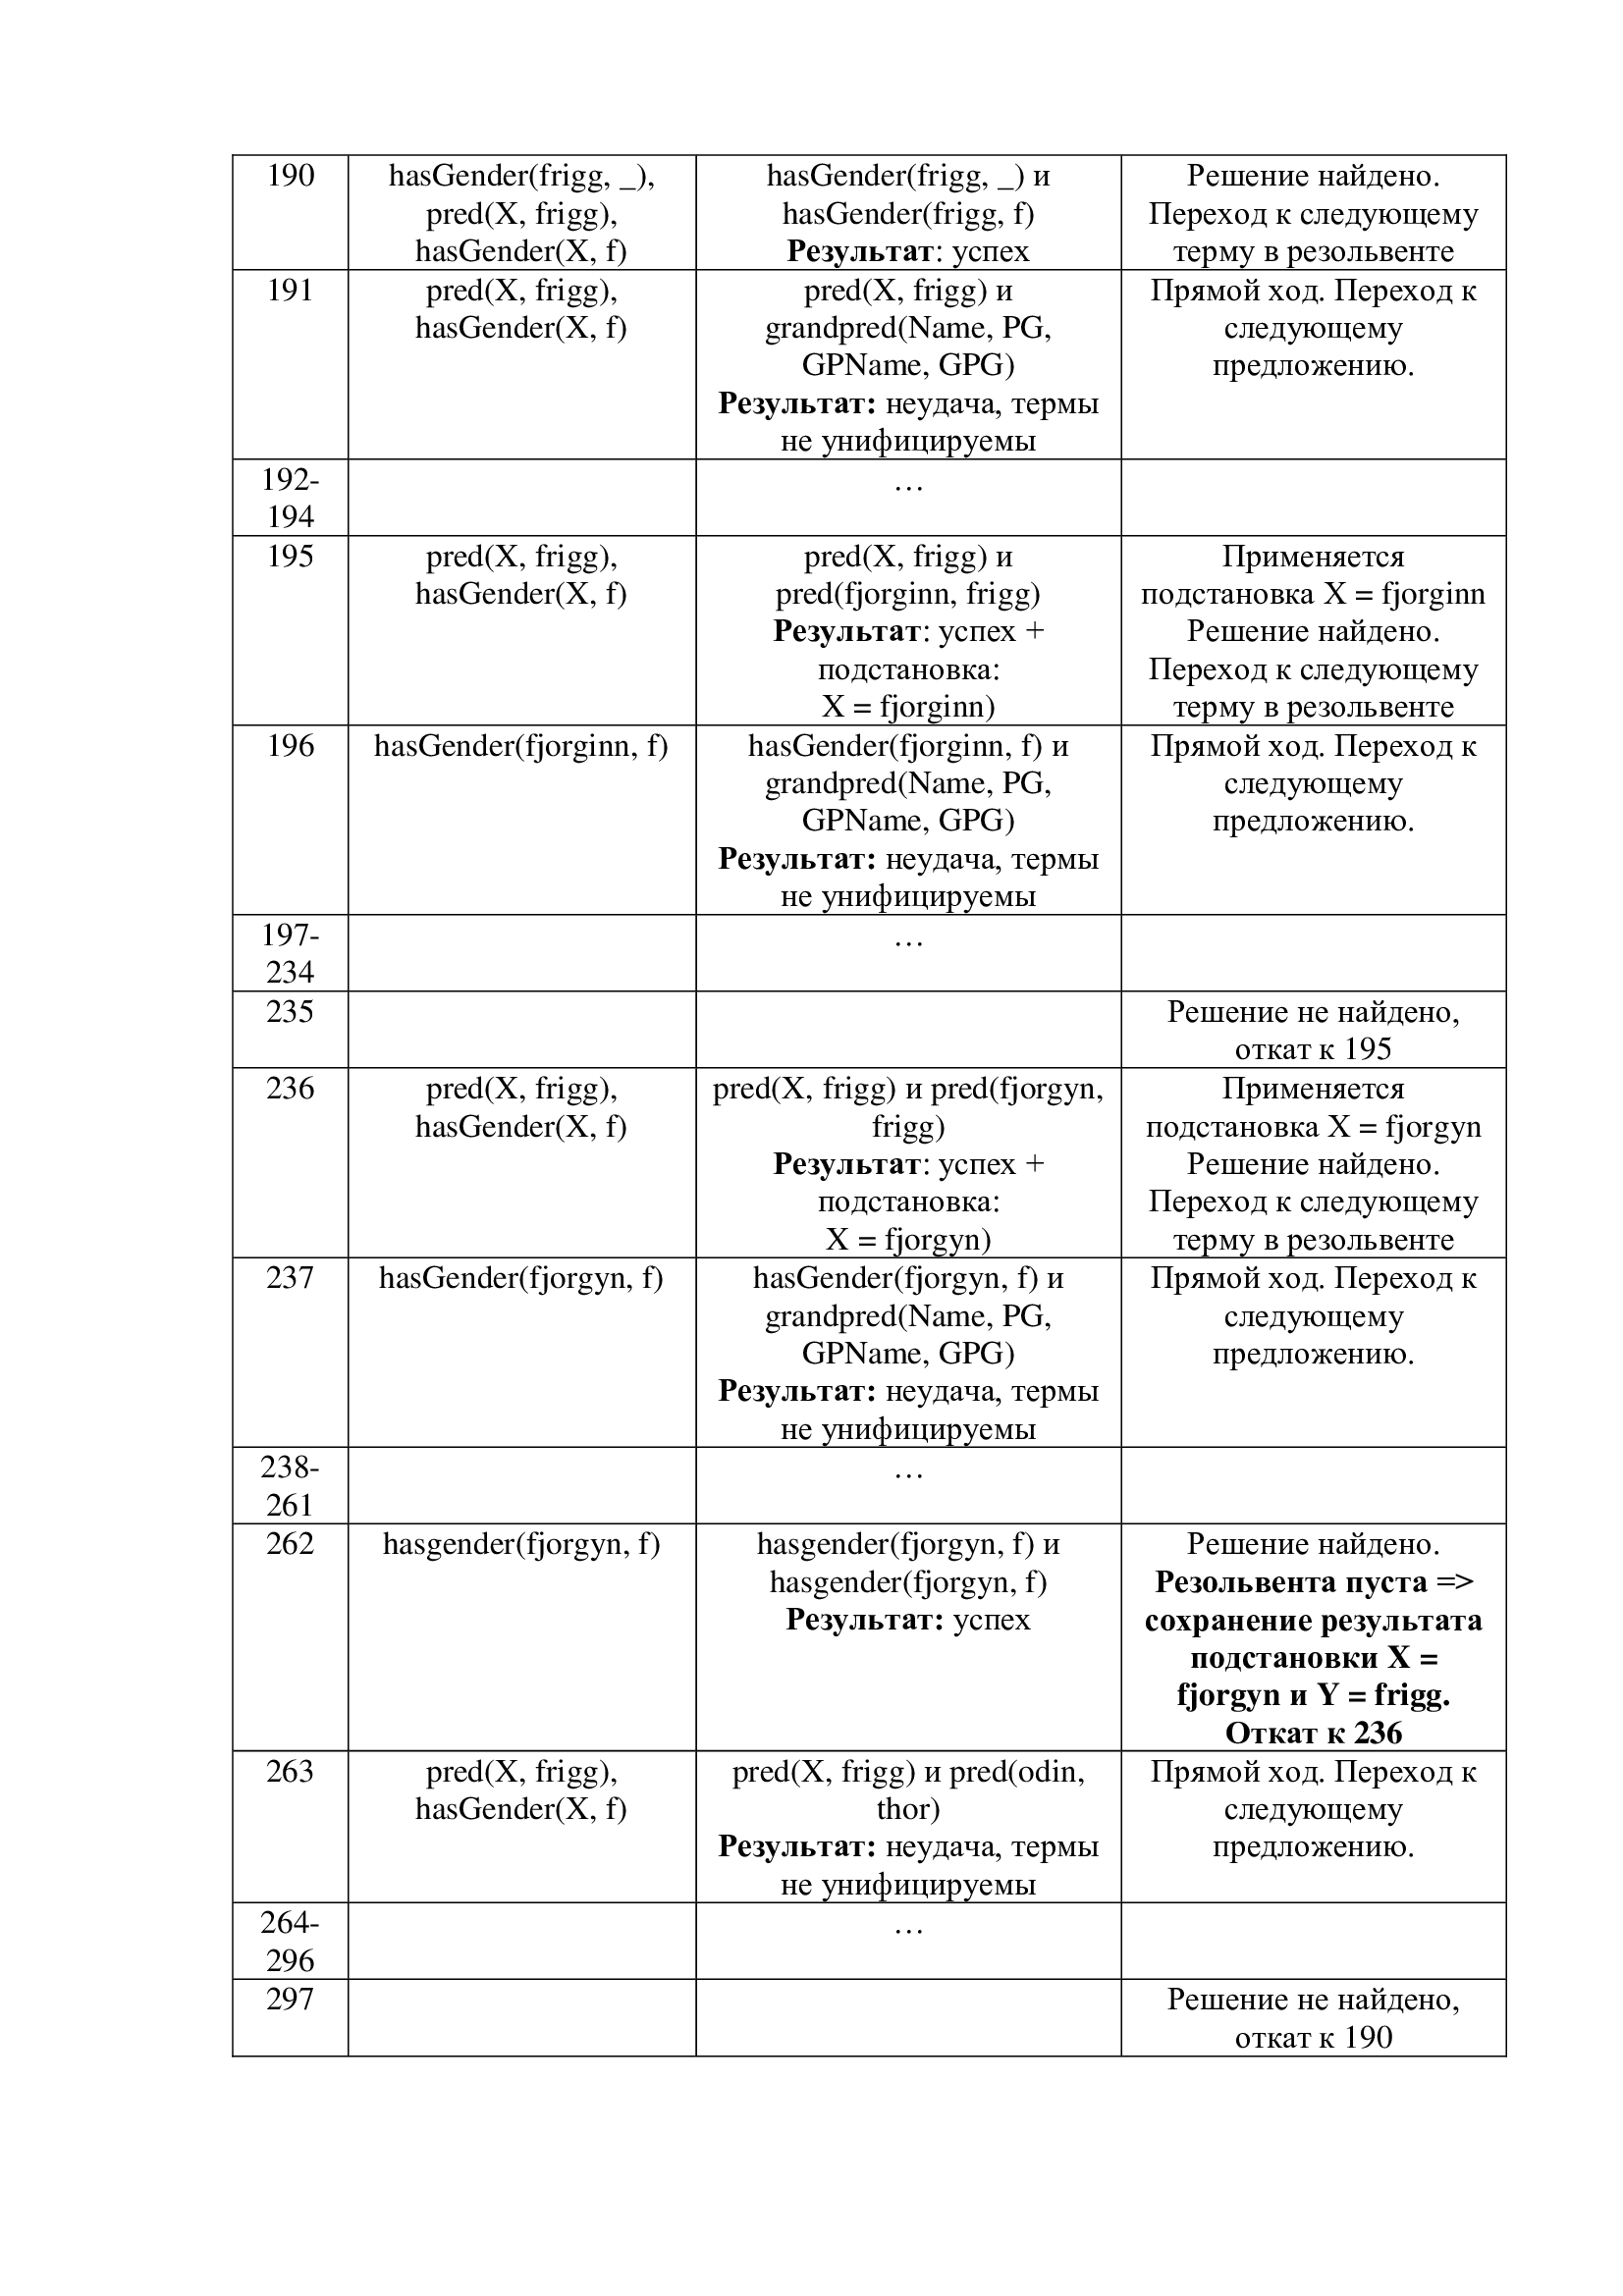
\includegraphics[scale=0.32]{2.png}
	\label{fig:2}
\end{figure}


\begin{figure}[H]
	\centering
	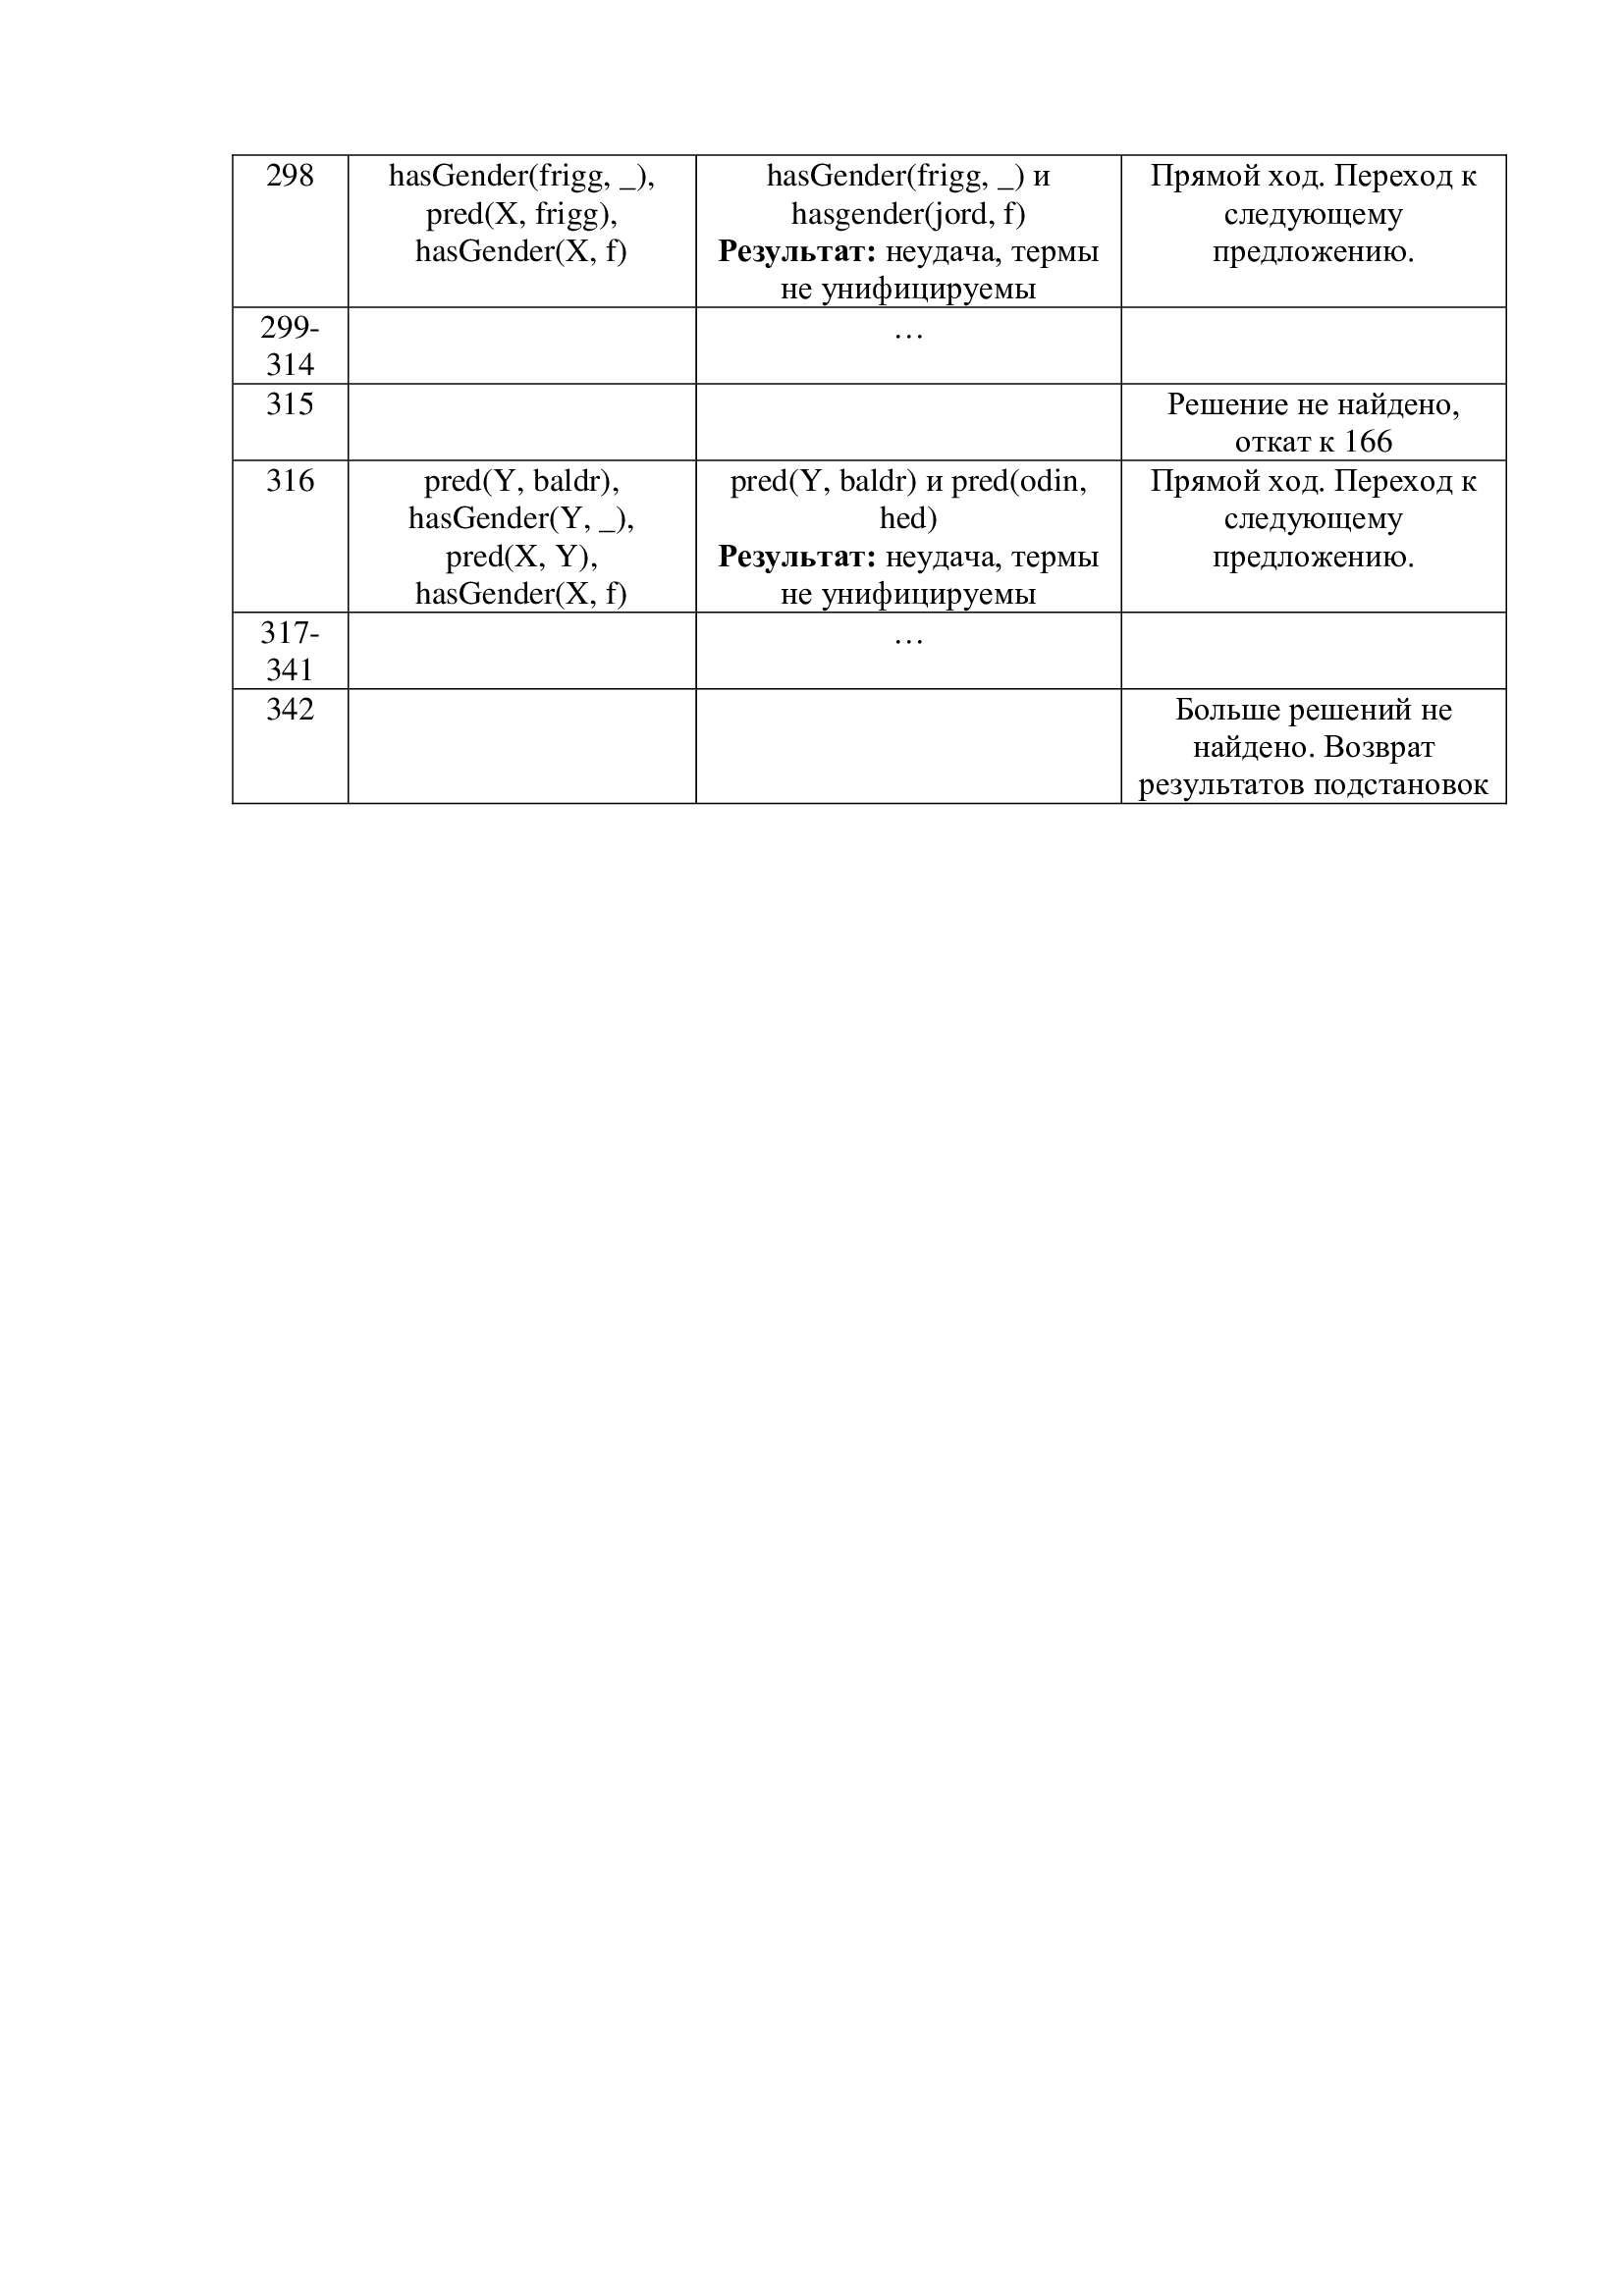
\includegraphics[scale=0.32]{3.png}
	\label{fig:2}
\end{figure}
\end{document}